\chapter{Batch Layer: Historical Storage and HBase Serving}
\label{chap:batch-layer}

\providecommand{\batchcell}[1]{\begin{minipage}[t]{\linewidth}#1\end{minipage}}
\providecommand{\scriptcell}[1]{\resizebox{\linewidth}{!}{\texttt{#1}}}
\providecommand{\tablehead}[1]{\textcolor{cmdcolor}{\textbf{#1}}}

\definecolor{cmdcolor}{RGB}{0,92,160}
\definecolor{tableblue}{RGB}{0,72,130}
\setlength{\arrayrulewidth}{0.45pt}


\newsavebox{\cmdboxcontent}
\newenvironment{cmdbox}{%
\par\smallskip\noindent\begingroup\setlength{\fboxsep}{4pt}%
\begin{lrbox}{\cmdboxcontent}%
\begin{minipage}{0.97\linewidth}\ttfamily\footnotesize\raggedright
}{%
\end{minipage}%
\end{lrbox}%
\fcolorbox{cmdcolor}{black!4}{\usebox{\cmdboxcontent}}%
\endgroup\par\smallskip
}


\sloppy

\section{Role of the Batch Layer}

The RAPID batch layer transforms the complete cybersecurity log corpus into reusable historical views. In a Lambda Architecture, this layer is not intended to produce immediate alerts, but rather to compute stable indicators from all available data \cite{marz2015bigdata}. It therefore complements the speed layer: streaming processing feeds Cassandra with the recent state, while batch processing rebuilds historical aggregations and exposes them through HBase.

Chawi's responsibility in this part mainly concerns the storage and serving of batch results. HDFS stores the source files and Parquet outputs that make it possible to replay or verify computations. HBase, hosted on Chawi's node at \texttt{100.97.208.110}, serves the historical views computed by Spark through the Thrift service on \texttt{9090}. This division respects the separation principle of the Lambda Architecture: HDFS remains the durable and rebuildable foundation, Spark produces the views, and HBase makes these views available to the API and the dashboard.

\section{Technical Objective and Processing Pipeline}

The technical objective of this layer is threefold. First, it stores the raw logs in HDFS in order to preserve a stable historical source. It then uses Spark to produce analytical views computed over the entire corpus. Finally, it materializes the aggregated results in HBase to enable fast reads by the API and the dashboard, without rerunning Spark jobs for each query.

The processing pipeline followed by RAPID is therefore as follows: raw logs are stored in HDFS, Spark batch jobs transform them into Parquet results under \texttt{/data/cybersecurity/batch}, and the serving-ready views are then inserted into HBase tables. The API and the dashboard subsequently consume these tables as the platform's historical memory. This logic justifies Chawi's contribution: HBase does not contain the raw logs, but query-oriented views ready to be served to application components.

Figure~\ref{fig:hdfs-ui-namenode} verifies that the NameNode Web interface is available. It confirms that HDFS is active and accessible before batch processing is executed.

\begin{cmdbox}
NameNode Web UI: http://\textless{}namenode\textgreater{}:9870
\end{cmdbox}

\begin{figure}[H]
    \centering
    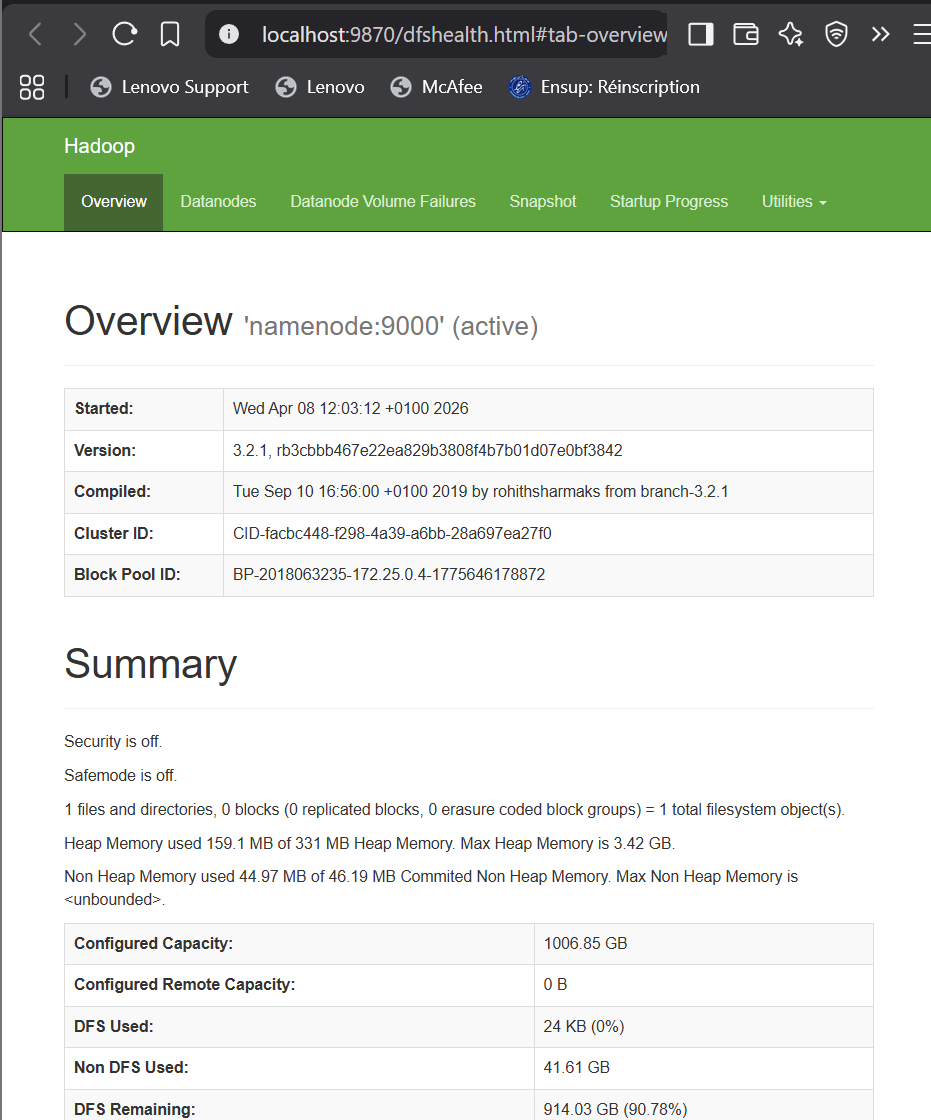
\includegraphics[width=0.7\textwidth]{figures/batch/hdfsUI1.png}
    \caption{HDFS Web interface showing the NameNode status and the availability of the distributed file system.}
    \label{fig:hdfs-ui-namenode}
\end{figure}

\section{HDFS Organization}

\subsection{Raw Partitions}

HDFS is used as durable storage for the raw logs \cite{hdfs_docs}. The project adopts a monthly partitioning convention under the \texttt{/logs} directory. The \texttt{/logs/year=2024/month=XX} area therefore corresponds to the raw input of the batch layer and the Kafka replay. It should not be confused with \texttt{/data/cybersecurity/batch}, which contains the analytical outputs.

Each month of the year 2024 has a \texttt{data.csv} file, for example:

\begin{itemize}
    \item \texttt{/logs/year=2024/month=01/data.csv}
    \item \texttt{/logs/year=2024/month=02/data.csv}
    \item \texttt{/logs/year=2024/month=12/data.csv}
\end{itemize}

This structure allows Spark batch jobs to read all months with the pattern \texttt{/logs/year=2024/month=*/data.csv}. It also allows the Kafka producer to replay the same partitions in the speed layer. The HDFS partitions therefore act as the source of truth: if an HBase or Cassandra table must be rebuilt, the computations can restart from the same monthly files.

The command below lists the monthly partitions under \texttt{/logs/year=2024}. This verification shows that the raw logs are organized by month, which makes it possible to process the full year or replay a specific period.

\begin{cmdbox}
docker exec -it namenode bash\\
hdfs dfs -ls /logs/year=2024
\end{cmdbox}

\begin{figure}[H]
    \centering
    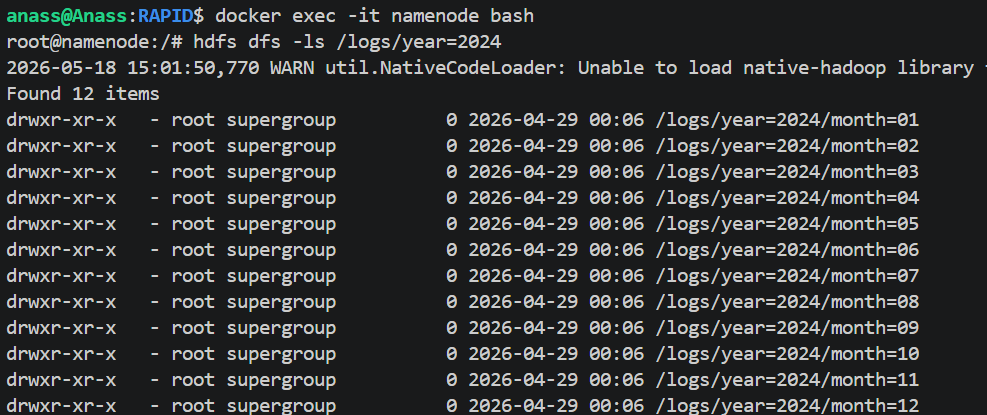
\includegraphics[width=\textwidth]{figures/batch/hdfspartition.png}
    \caption{Partitioning of raw logs in HDFS by year and month.}
    \label{fig:hdfs-raw-partitioning}
\end{figure}

\subsection{Batch Outputs}

Historical outputs are written under \texttt{/data/cybersecurity/batch}. The Spark scripts in \texttt{spark/batch/} generally write two forms of output: a Parquet output in HDFS for audit and reconstruction, then an HBase table for serving the aggregated views. Table~\ref{tab:hdfs-batch-outputs} summarizes the paths observed in the project.

\begingroup
\footnotesize
\setlength{\tabcolsep}{5pt}
\renewcommand{\arraystretch}{1.32}
\begin{longtable}{|
    >{\raggedright\arraybackslash\bfseries}p{0.24\textwidth}|
    >{\raggedright\arraybackslash}p{0.34\textwidth}|
    >{\raggedright\arraybackslash}p{0.30\textwidth}|
}
    \caption{Batch outputs produced in HDFS.}
    \label{tab:hdfs-batch-outputs}\\
    \hline
    \tablehead{Spark Job} & \tablehead{HDFS Path} & \tablehead{Role of the Result} \\
    \hline
    \endfirsthead
    \hline
    \tablehead{Spark Job} & \tablehead{HDFS Path} & \tablehead{Role of the Result} \\
    \hline
    \endhead
    \batchcell{\scriptcell{top10\_malicious\_ips.py}} &
    \batchcell{\texttt{/data/cybersecurity/}\\\texttt{batch/top10\_malicious\_ips}} &
    Ranking of the most dangerous source IPs and basis for the historical reputation score. \\
    \hline

    \batchcell{\scriptcell{attack\_path\_analysis.py}} &
    \batchcell{\texttt{/data/cybersecurity/}\\\texttt{batch/attack\_patterns}} &
    Aggregation of SQLi, XSS, Path Traversal and ToolScan patterns by attack type and threat label. \\
    \hline

    \batchcell{\scriptcell{hbase\_threat\_timeline.py}} &
    \batchcell{\texttt{/data/cybersecurity/}\\\texttt{batch/threat\_timeline/}\\\texttt{hourly}\\\texttt{/data/cybersecurity/}\\\texttt{batch/threat\_timeline/}\\\texttt{daily}} &
    Hourly and daily event time series by threat level. \\
    \hline

    \batchcell{\scriptcell{port\_scan\_detection.py}} &
    \batchcell{\texttt{/data/cybersecurity/}\\\texttt{batch/port\_scans}} &
    Five-minute windows in which a source IP contacts more than twenty distinct ports. \\
    \hline

    \batchcell{\scriptcell{volume\_by\_threat.py}} &
    \batchcell{\texttt{/data/cybersecurity/}\\\texttt{batch/volume\_by\_threat}} &
    Network volume statistics by \texttt{threat\_label}, including mean, maximum, standard deviation and 95th percentile. \\
    \hline

    \batchcell{\scriptcell{multistep\_attack\_detection.py}} &
    \batchcell{\texttt{/data/cybersecurity/}\\\texttt{batch/views/}\\\texttt{multistep\_attacks}} &
    Enriched view of IPs that combine reconnaissance, SQLi exploitation and Path Traversal. \\
    \hline

    Intermediate view &
    \batchcell{\texttt{/data/cybersecurity/}\\\texttt{batch/classified\_attacks}} &
    Parquet input expected by the multi-step detector to group already classified attacks. \\
    \hline
\end{longtable}
\endgroup

This organization clearly separates raw files, analytical outputs, and serving-ready views. Parquet files do not replace HBase: they serve as a technical trace and as support for recomputation. HBase receives only the aggregations required for fast reads.

The following commands show the global \texttt{/data/cybersecurity} directory and then the batch output folders. The result validates the presence of views generated by Spark, including \texttt{attack\_patterns}, \texttt{port\_scans}, \texttt{threat\_timeline}, \texttt{top\_malicious\_ips}, \texttt{views} and \texttt{volume\_by\_threat}.

\begin{cmdbox}
hdfs dfs -ls /data/cybersecurity\\
hdfs dfs -ls /data/cybersecurity/batch
\end{cmdbox}

\begin{figure}[H]
    \centering
    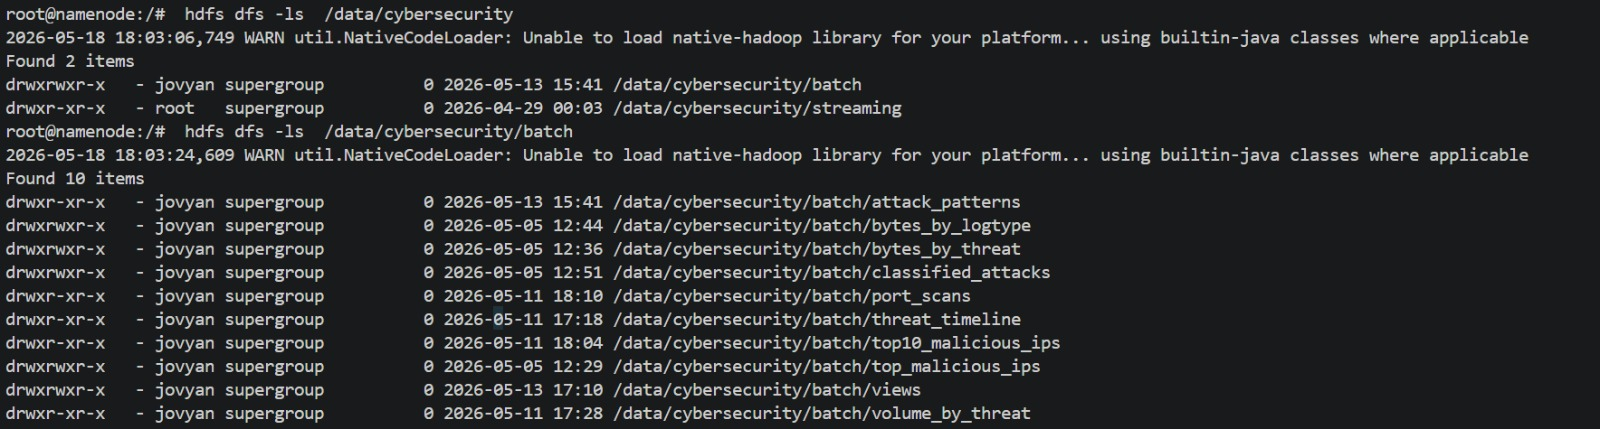
\includegraphics[width=\textwidth]{figures/batch/spark_batch_output_folders_and_directory_structure.jpeg}
    \caption{HDFS directories containing the outputs generated by Spark batch processing.}
    \label{fig:spark-batch-output-folders}
\end{figure}

\subsection{HDFS Storage Zones}

The separation of HDFS zones clarifies the role of each directory. The \texttt{/logs/year=2024/month=XX} zone corresponds to raw inputs, while \texttt{/data/cybersecurity/batch} corresponds to analytical results. The \texttt{/data/cybersecurity/streaming} zone may exist in the tree, but it is not the main scope of this chapter.

\begingroup
\footnotesize
\setlength{\tabcolsep}{5pt}
\renewcommand{\arraystretch}{1.28}
\begin{longtable}{|
    >{\raggedright\arraybackslash\bfseries}p{0.33\textwidth}|
    >{\raggedright\arraybackslash}p{0.24\textwidth}|
    >{\raggedright\arraybackslash}p{0.31\textwidth}|
}
    \caption{HDFS zones used by the batch layer.}
    \label{tab:hdfs-storage-zones}\\
    \hline
    \tablehead{HDFS Zone} & \tablehead{Content} & \tablehead{Usage} \\
    \hline
    \endfirsthead
    \hline
    \tablehead{HDFS Zone} & \tablehead{Content} & \tablehead{Usage} \\
    \hline
    \endhead
    \batchcell{\texttt{/logs/year=2024/}\\\texttt{month=XX}} &
    Partitioned raw logs &
    Batch source and Kafka replay \\
    \hline

    \batchcell{\texttt{/data/cybersecurity/}\\\texttt{batch}} &
    Parquet outputs &
    Audit, verification and reconstruction \\
    \hline

    \batchcell{\texttt{/data/cybersecurity/}\\\texttt{batch/views}} &
    Analytical views &
    Results prepared for exploitation \\
    \hline

    \batchcell{\texttt{/data/cybersecurity/}\\\texttt{streaming}} &
    Possible streaming outputs &
    Outside the main scope of the batch chapter \\
    \hline
\end{longtable}
\endgroup

\section{Batch Job Input Schema}

Batch jobs use an explicit schema to avoid automatic inference and maintain a stable data contract with HDFS. This contract is consistent with the architecture chapter: the same attributes feed batch processing, Kafka replay, and serving views.

\begingroup
\small
\setlength{\tabcolsep}{5pt}
\renewcommand{\arraystretch}{1.28}
\begin{longtable}{|
    >{\raggedright\arraybackslash\bfseries}p{0.24\textwidth}|
    >{\raggedright\arraybackslash}p{0.64\textwidth}|
}
    \caption{Input schema of batch processing.}
    \label{tab:batch-input-schema}\\
    \hline
    \tablehead{Field} & \tablehead{Analytical Role} \\
    \hline
    \endfirsthead
    \hline
    \tablehead{Field} & \tablehead{Analytical Role} \\
    \hline
    \endhead
    \texttt{timestamp} & Event time, used for windows and historical series. \\
    \hline
    \texttt{source\_ip} & Source address used for reputation, scans and correlations. \\
    \hline
    \texttt{dest\_ip} & Network target observed in the log. \\
    \hline
    \texttt{protocol} & Network protocol, useful for filtering certain behaviors such as TCP scans. \\
    \hline
    \texttt{action} & Observed action, for example an allowed or blocked request. \\
    \hline
    \texttt{threat\_label} & Threat class used for historical aggregations. \\
    \hline
    \texttt{log\_type} & Log category, useful for qualifying the source of the event. \\
    \hline
    \scriptcell{bytes\_transferred} & Network volume used in traffic statistics. \\
    \hline
    \texttt{user\_agent} & Field used to detect ToolScan and certain offensive tool signatures. \\
    \hline
    \texttt{request\_path} & HTTP path used to detect SQLi, XSS and Path Traversal. \\
    \hline
\end{longtable}
\endgroup

Spark reads HDFS partitions with an \textit{HDFS-first} strategy. If HDFS is unavailable during a development run, the scripts provide a local fallback to the local path \texttt{/home/jovyan/work/batch/}\linebreak[1]\texttt{cybersecurity\_threat\_detection\_logs.csv}. In the RAPID deployment, however, the HDFS path remains the nominal path, because it makes it possible to process the full year and rebuild outputs reproducibly \cite{spark_docs}.

\subsection{Spark Batch Scripts and Responsibilities}

The scripts in the \texttt{spark/batch/} folder materialize the analytical logic of the batch layer. Each script reads the historical logs, builds a specialized view, and then writes the result either as Parquet in HDFS or into HBase when the view must be consumed quickly by the service. This dual output provides technical traceability: HDFS makes it possible to verify and rebuild computations, while HBase exposes the results as directly queryable rows.

The \texttt{ml\_bonus.py} script is treated as an experimental complement: it locally trains a Random Forest model on simple features and saves local predictions. It is therefore not central to HBase serving, unlike the scripts that feed the \texttt{ip\_reputation}, \texttt{attack\_patterns}, \texttt{threat\_timeline}, \texttt{port\_scans}, \texttt{threat\_volume} and \texttt{multistep\_attacks} tables.

\begingroup
\scriptsize
\setlength{\tabcolsep}{4pt}
\renewcommand{\arraystretch}{1.34}
\begin{longtable}{|
    >{\raggedright\arraybackslash\bfseries}p{0.23\textwidth}|
    >{\raggedright\arraybackslash}p{0.42\textwidth}|
    >{\raggedright\arraybackslash}p{0.25\textwidth}|
}
    \caption{Summary of Spark batch scripts and produced views.}
    \label{tab:spark-batch-scripts}\\
    \hline
    \tablehead{Script} & \tablehead{Processing Performed} & \tablehead{HDFS Output / HBase Table} \\
    \hline
    \endfirsthead
    \hline
    \tablehead{Script} & \tablehead{Processing Performed} & \tablehead{HDFS Output / HBase Table} \\
    \hline
    \endhead

    \batchcell{\scriptcell{top10\_malicious\_ips.py}} &
    Ranks source IPs whose \texttt{threat\_label} is \texttt{suspicious} or \texttt{malicious}. The script adds SQLi, XSS, Path Traversal and ToolScan indicators, then computes a \texttt{reputation\_score} normalized between 0 and 100. &
    \batchcell{\texttt{batch/top10\_}\\\texttt{malicious\_ips}\\[1mm]\texttt{ip\_reputation}} \\
    \hline

    \batchcell{\scriptcell{attack\_path\_analysis.py}} &
    Analyzes \texttt{request\_path} and \texttt{user\_agent} with SQLi, XSS, Path Traversal and ToolScan signatures. It aggregates occurrences, volumes, distinct IPs and the latest observation by attack type and threat level. &
    \batchcell{\texttt{batch/attack\_}\\\texttt{patterns}\\[1mm]\texttt{attack\_patterns}} \\
    \hline

    \batchcell{\scriptcell{hbase\_threat\_timeline.py}} &
    Produces an hourly and daily historical timeline. The aggregates store the number of events, the number of distinct IPs and the total volume by \texttt{threat\_label}. &
    \batchcell{\texttt{batch/threat\_}\\\texttt{timeline/hourly}\\\texttt{batch/threat\_}\\\texttt{timeline/daily}\\[1mm]\texttt{threat\_timeline}} \\
    \hline

    \batchcell{\scriptcell{port\_scan\_detection.py}} &
    Filters TCP logs, extracts the destination port and detects sources that contact more than twenty distinct ports within a five-minute window. &
    \batchcell{\texttt{batch/port\_scans}\\[1mm]\texttt{port\_scans}} \\
    \hline

    \batchcell{\scriptcell{volume\_by\_threat.py}} &
    Correlates \texttt{bytes\_transferred} with \texttt{threat\_label}. The script computes the number of events, the mean, minimum, maximum and total volumes, the standard deviation and the 95th percentile. &
    \batchcell{\texttt{batch/volume\_}\\\texttt{by\_threat}\\[1mm]\texttt{threat\_volume}} \\
    \hline

    \batchcell{\scriptcell{multistep\_attack\_detection.py}} &
    Reads the \texttt{classified\_attacks} view and searches for IPs that combine ToolScan, SQLi and Path Traversal. It enriches each IP with counters, average volume, the number of malicious events and a \texttt{risk\_level}. &
    \batchcell{\texttt{batch/views/}\\\texttt{multistep\_attacks}\\[1mm]\texttt{multistep\_attacks}} \\
    \hline

    \batchcell{\texttt{ml\_bonus.py}} &
    Local bonus script. It trains a Random Forest on \texttt{bytes\_transferred}, \texttt{protocol}, \texttt{action} and \texttt{log\_type}, evaluates accuracy, F1, precision and recall, then saves the predictions. &
    \batchcell{\texttt{./data/}\\\texttt{predictions.parquet}\\[1mm]No HBase table} \\
    \hline
\end{longtable}
\endgroup

\section{Historical Serving with HBase}

\subsection{Modeling Principle}

HBase is used as a historical serving store because its model based on rows, column families and sortable keys is suitable for reads by identifier or by temporal prefix \cite{hbase_docs}. Batch jobs connect to Chawi's Thrift service with HappyBase and write the results into HBase tables. The operational contract observed in the batch scripts uses the \texttt{cf} column family; the column qualifiers then carry the metrics computed by each job.

The HBase list verifies that the serving tables exist before the API or the dashboard queries them. This output illustrates the historical tables used by the batch layer: \texttt{attack\_patterns}, \texttt{ip\_reputation}, \texttt{multistep\_attacks}, \texttt{port\_scans}, \texttt{threat\_timeline} and \texttt{threat\_volume}.

\begin{cmdbox}
docker exec -it hbase hbase shell\\
list
\end{cmdbox}

\begin{figure}[H]
    \centering
    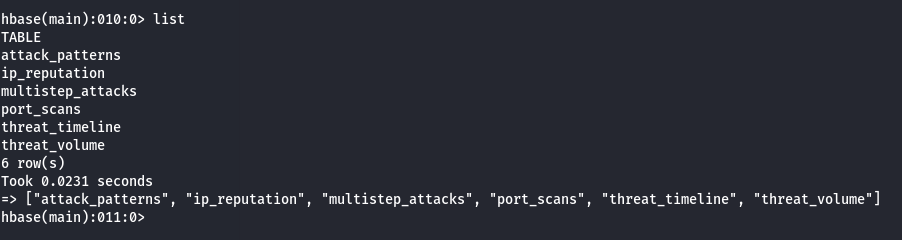
\includegraphics[width=\textwidth]{figures/batch/hbase_tables_list.png}
    \caption{List of HBase tables used to serve historical batch results.}
    \label{fig:hbase-tables-list}
\end{figure}

The HBase creation script initializes the main IP reputation, attack pattern and threat timeline tables. The batch scripts present in the project also add specialized tables for port scans, traffic volumes and multi-step attacks. These tables are documented here because they belong to the same batch/HBase contract found in the repository.

\subsection{HBase Modeling Choices}

HBase is not used to store raw logs. The complete logs remain in HDFS, while HBase contains aggregated views ready to be served. This choice reduces the volume read by the API and makes responses more direct for the dashboard.

The row key is chosen according to the expected query pattern: \texttt{source\_ip} for reputation, \texttt{HOURLY|heure|threat\_label} or \texttt{DAILY|jour|threat\_label} for the timeline, \texttt{source\_ip|window\_start} for port scans, and \texttt{THREAT\_VOL|threat\_label} for volume statistics. The \texttt{cf} column family groups the metrics computed by Spark, keeping the model simple and consistent across tables.

\subsection{HBase Tables of the Batch Layer}

Table~\ref{tab:hbase-batch-schemas} details the HBase schemas used to serve historical results. Row keys are chosen to match expected access patterns: an IP for reputation, an attack type for patterns, a temporal prefix for series, or an observation window for port scans.

\begingroup
\scriptsize
\setlength{\tabcolsep}{4pt}
\renewcommand{\arraystretch}{1.34}
\begin{longtable}{|
    >{\raggedright\arraybackslash\bfseries}p{0.15\textwidth}|
    >{\raggedright\arraybackslash}p{0.24\textwidth}|
    >{\raggedright\arraybackslash}p{0.39\textwidth}|
}
    \caption{HBase schemas of batch views.}
    \label{tab:hbase-batch-schemas}\\
    \hline
    \tablehead{Table} & \tablehead{Row Key and Producer} & \tablehead{Main Columns} \\
    \hline
    \endfirsthead
    \hline
    \tablehead{Table} & \tablehead{Row Key and Producer} & \tablehead{Main Columns} \\
    \hline
    \endhead

    \texttt{ip\_reputation} &
    \batchcell{\texttt{source\_ip}\\\texttt{top10\_malicious\_ips.py}} &
    \batchcell{\texttt{cf:threat\_count}, \texttt{cf:sqli\_hits}, \texttt{cf:xss\_hits},\\
    \texttt{cf:traversal\_hits}, \texttt{cf:tool\_hits}, \texttt{cf:avg\_bytes},\\
    \texttt{cf:reputation\_score}} \\
    \hline

    \batchcell{\texttt{attack\_}\\\texttt{patterns}} &
    \batchcell{\texttt{attack\_type|}\\\texttt{threat\_label}\\\texttt{attack\_path\_}\\\texttt{analysis.py}} &
    \batchcell{\texttt{cf:attack\_type}, \texttt{cf:threat\_label}, \texttt{cf:occurrences},\\
    \texttt{cf:avg\_bytes}, \texttt{cf:total\_bytes}, \texttt{cf:distinct\_ips},\\
    \texttt{cf:last\_seen}} \\
    \hline

    \batchcell{\texttt{threat\_}\\\texttt{timeline}} &
    \batchcell{\texttt{HOURLY|heure|}\\\texttt{threat\_label}\\\texttt{DAILY|jour|}\\\texttt{threat\_label}\\\texttt{hbase\_threat\_}\\\texttt{timeline.py}} &
    \batchcell{\texttt{cf:heure} or \texttt{cf:jour}, \texttt{cf:threat\_label},\\
    \texttt{cf:event\_count}, \texttt{cf:distinct\_ips}, \texttt{cf:total\_bytes}} \\
    \hline

    \texttt{port\_scans} &
    \batchcell{\texttt{source\_ip|}\\\texttt{window\_start}\\\texttt{port\_scan\_detection.py}} &
    \batchcell{\texttt{cf:source\_ip}, \texttt{cf:distinct\_ports},\\
    \texttt{cf:total\_connections}, \texttt{cf:window\_start}, \texttt{cf:window\_end}} \\
    \hline

    \texttt{threat\_volume} &
    \batchcell{\texttt{THREAT\_VOL|}\\\texttt{threat\_label}\\\texttt{volume\_by\_threat.py}} &
    \batchcell{\texttt{cf:threat\_label}, \texttt{cf:total\_bytes}, \texttt{cf:avg\_bytes},\\
    \texttt{cf:min\_bytes}, \texttt{cf:max\_bytes}, \texttt{cf:stddev\_bytes},\\
    \texttt{cf:p95\_bytes}, \texttt{cf:count}} \\
    \hline

    \batchcell{\texttt{multistep\_}\\\texttt{attacks}} &
    \batchcell{\texttt{source\_ip}\\\scriptcell{multistep\_attack\_detection.py}} &
    \batchcell{\texttt{cf:total\_events}, \texttt{cf:attack\_types}, \texttt{cf:sqli\_hits},\\
    \texttt{cf:traversal\_hits}, \texttt{cf:tool\_hits}, \texttt{cf:avg\_bytes},\\
    \texttt{cf:malicious\_count}, \texttt{cf:risk\_level}} \\
    \hline
\end{longtable}
\endgroup

\begingroup
\small
\setlength{\tabcolsep}{5pt}
\renewcommand{\arraystretch}{1.28}
\begin{longtable}{|
    >{\raggedright\arraybackslash\bfseries}p{0.29\textwidth}|
    >{\raggedright\arraybackslash}p{0.59\textwidth}|
}
    \caption{API/dashboard usage of batch views.}
    \label{tab:hbase-frontend-usage}\\
    \hline
    \tablehead{HBase Table} & \tablehead{Service/dashboard Usage} \\
    \hline
    \endfirsthead
    \hline
    \tablehead{HBase Table} & \tablehead{Service/dashboard Usage} \\
    \hline
    \endhead
    \texttt{ip\_reputation} & Historical score and reputation detail by IP. \\
    \hline
    \texttt{attack\_patterns} & Distribution of detected attack families. \\
    \hline
    \texttt{threat\_timeline} & Chronological threat chart. \\
    \hline
    \texttt{port\_scans} & Detected scan behaviors. \\
    \hline
    \texttt{threat\_volume} & Volume chart and statistics by threat level. \\
    \hline
    \texttt{multistep\_attacks} & Advanced multi-step correlation view. \\
    \hline
\end{longtable}
\endgroup

\subsection{\texttt{ip\_reputation}}

The \texttt{ip\_reputation} table is the historical view most directly used by the service. Each row represents a source IP and groups the signals observed across the complete history: average volume, reputation score, SQLi, XSS and Path Traversal indicators, offensive tools and number of threatening events. The expected query is a direct read by \texttt{source\_ip}.

The HBase command below verifies the table schema and displays a sample of served rows. It shows that historical reputation is materialized by IP with \texttt{avg\_bytes}, \texttt{reputation\_score}, \texttt{sqli\_hits}, \texttt{threat\_count}, \texttt{tool\_hits}, \texttt{traversal\_hits} and \texttt{xss\_hits}.

\begin{cmdbox}
describe 'ip\_reputation'\\
scan 'ip\_reputation', \{LIMIT =\textgreater{} 5\}
\end{cmdbox}

\begin{figure}[H]
    \centering
    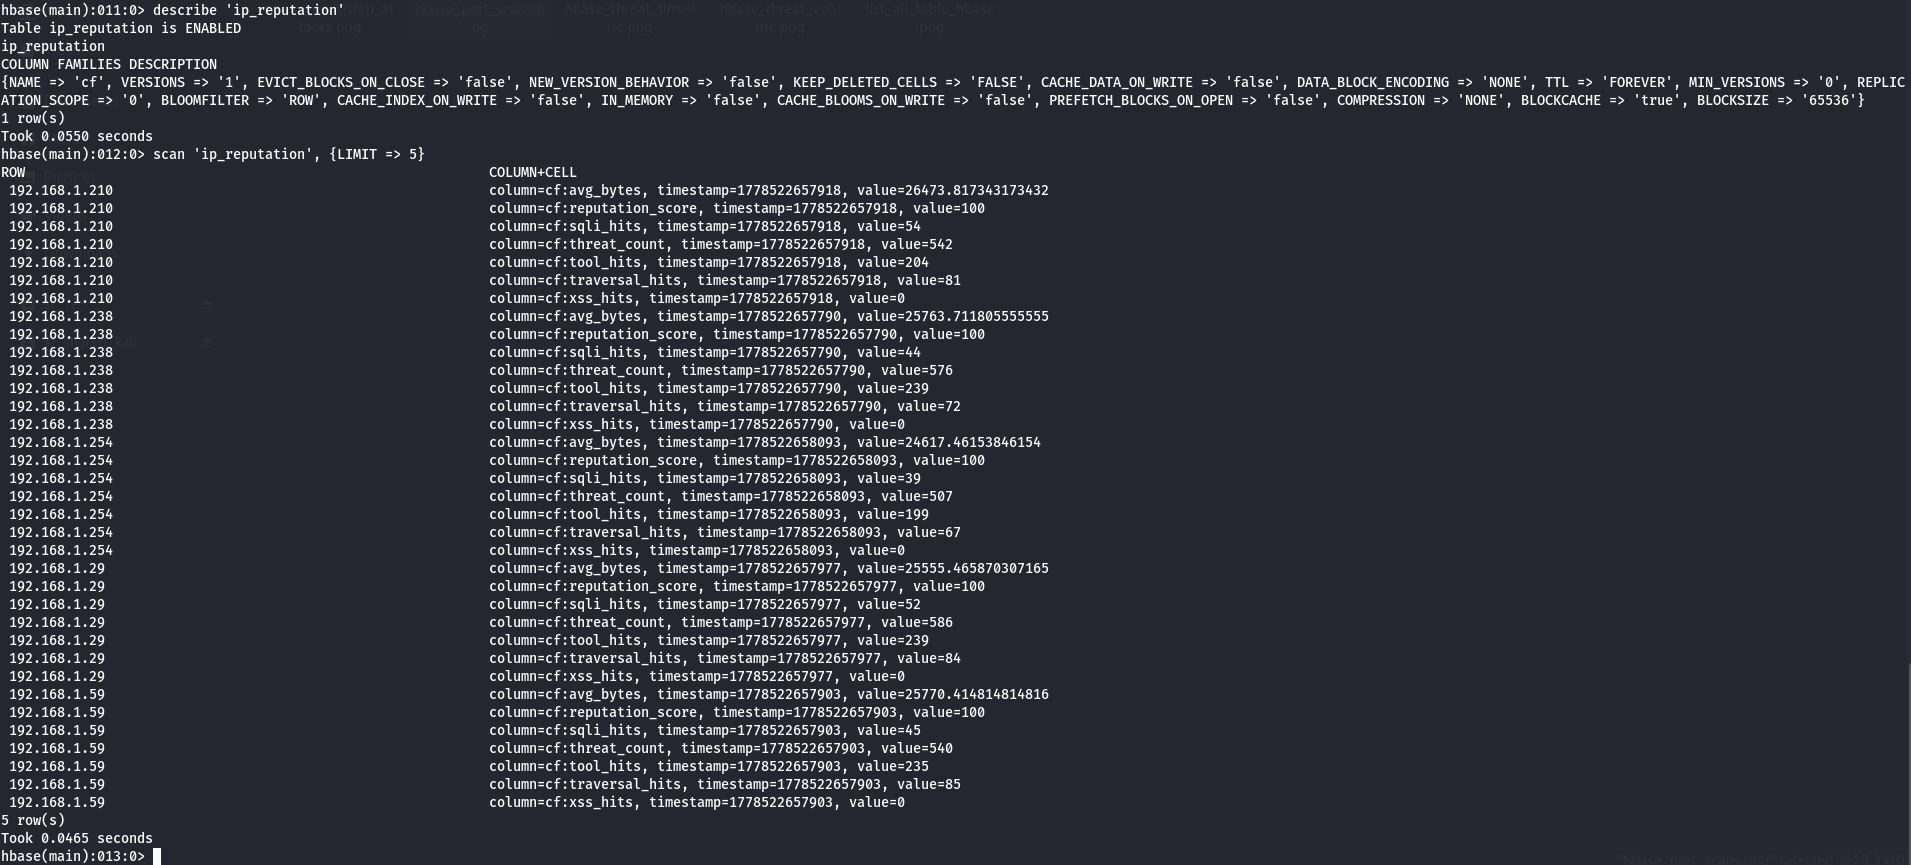
\includegraphics[width=\textwidth]{figures/batch/hbase_ip_reputation.png}
    \caption{Schema and sample rows of the HBase \texttt{ip\_reputation} table.}
    \label{fig:hbase-ip-reputation}
\end{figure}

This table allows the API to complement the real-time state with historical memory. When a client requests \texttt{/threats/ip/<ip>}, the API reads the HBase row associated with the IP and compares this historical signal with Cassandra scores in order to produce a single decision for the dashboard.

\subsection{\texttt{attack\_patterns}}

The \texttt{attack\_patterns} table stores the attack patterns extracted from HTTP paths and user agents. The path analysis job classifies events with regular expressions for SQLi, XSS, Path Traversal and ToolScan. The composite key associates the attack type with the threat level, making each combination directly addressable and avoiding an overly wide row per attack type. The expected read is by attack family and by \texttt{threat\_label} to build an aggregated distribution.

The \texttt{cf:occurrences}, \texttt{cf:distinct\_ips}, \texttt{cf:total\_bytes}, \texttt{cf:avg\_bytes} and \texttt{cf:last\_seen} columns provide a synthetic view of historical behavior. This modeling is useful for explaining which attack families dominate the corpus and for feeding aggregated visualizations without rereading all HDFS files.

\subsection{\texttt{threat\_timeline}}

The \texttt{threat\_timeline} table serves temporal trends. The HBase timeline job produces an hourly and daily historical evolution, separated by \texttt{threat\_label}. The expected read is by period and by threat label in order to feed a temporal chart.

The following commands verify the table schema and display sample rows. This verification shows that the table stores the daily evolution by label with \texttt{event\_count}, \texttt{distinct\_ips}, \texttt{total\_bytes}, \texttt{jour} and \texttt{threat\_label}.

\begin{cmdbox}
describe 'threat\_timeline'\\
scan 'threat\_timeline', \{LIMIT =\textgreater{} 5\}
\end{cmdbox}

\begin{figure}[H]
    \centering
    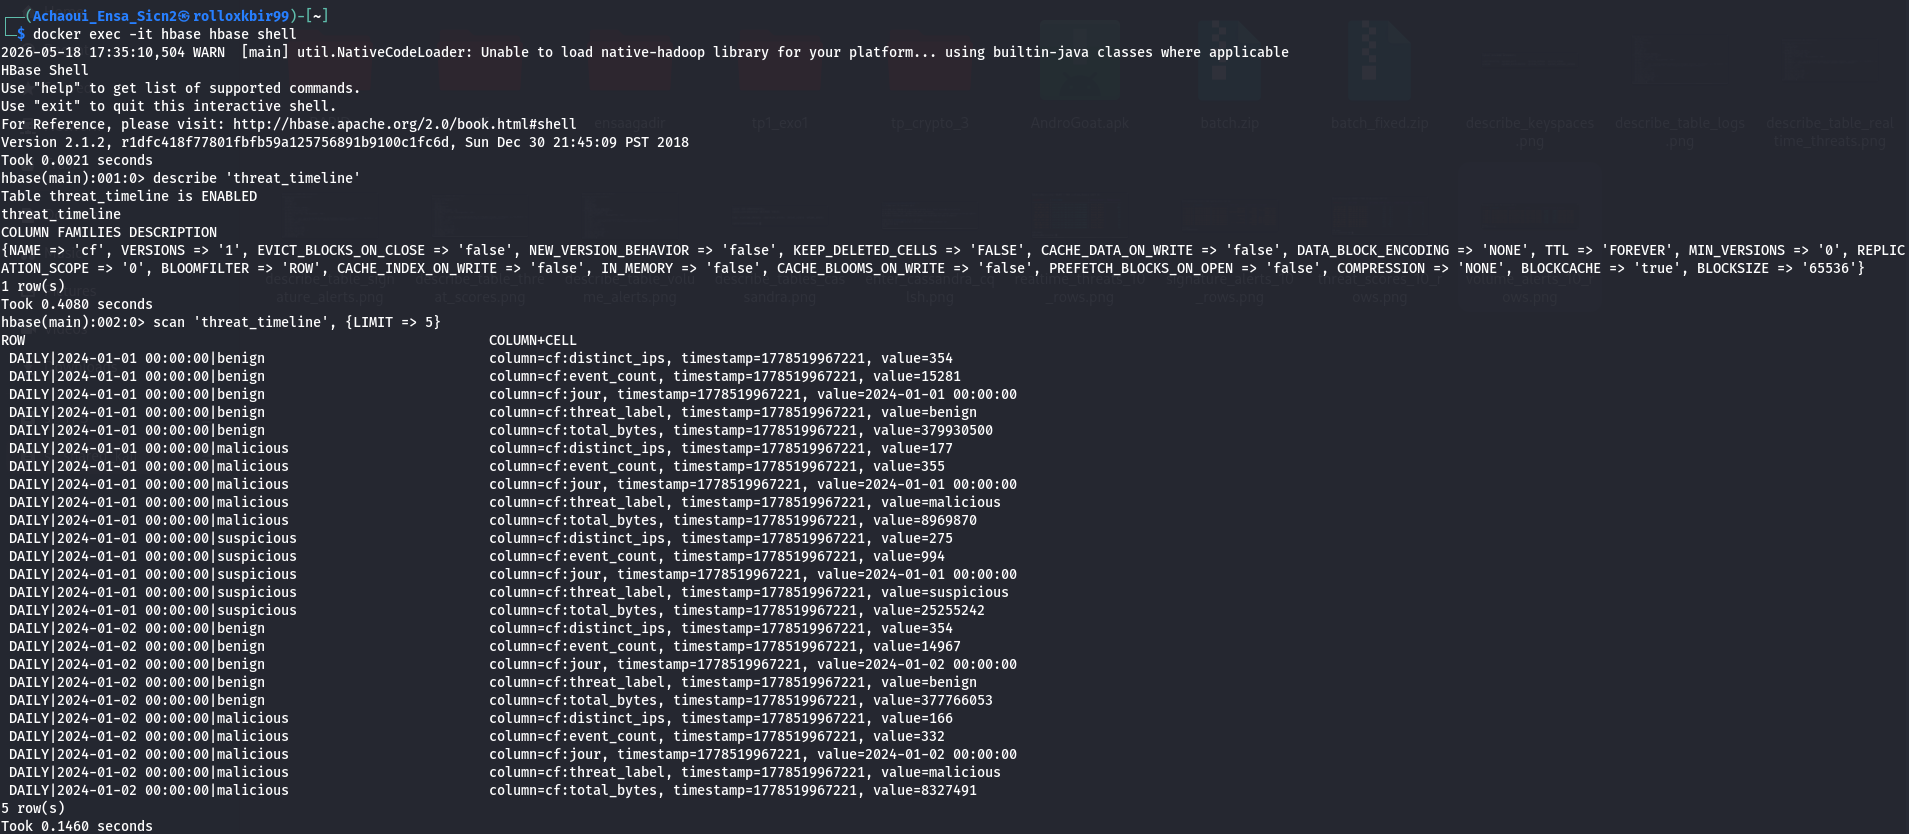
\includegraphics[width=\textwidth]{figures/batch/hbase_threat_timeline.png}
    \caption{Schema and sample rows of the HBase \texttt{threat\_timeline} table.}
    \label{fig:hbase-threat-timeline}
\end{figure}

\subsection{\texttt{port\_scans}}

The \texttt{port\_scans} table stores the windows where a TCP source contacts a high number of distinct ports. Each row associates a source IP with a time window and stores the counters required to directly serve port scan detection results. The expected read is by \texttt{source\_ip} and \texttt{window\_start}.

The HBase output confirms that scan aggregations are materialized. It exposes the \texttt{source\_ip}, \texttt{distinct\_ports}, \texttt{total\_connections}, \texttt{window\_start} and \texttt{window\_end} columns.

\begin{cmdbox}
describe 'port\_scans'\\
scan 'port\_scans', \{LIMIT =\textgreater{} 5\}
\end{cmdbox}

\begin{figure}[H]
    \centering
    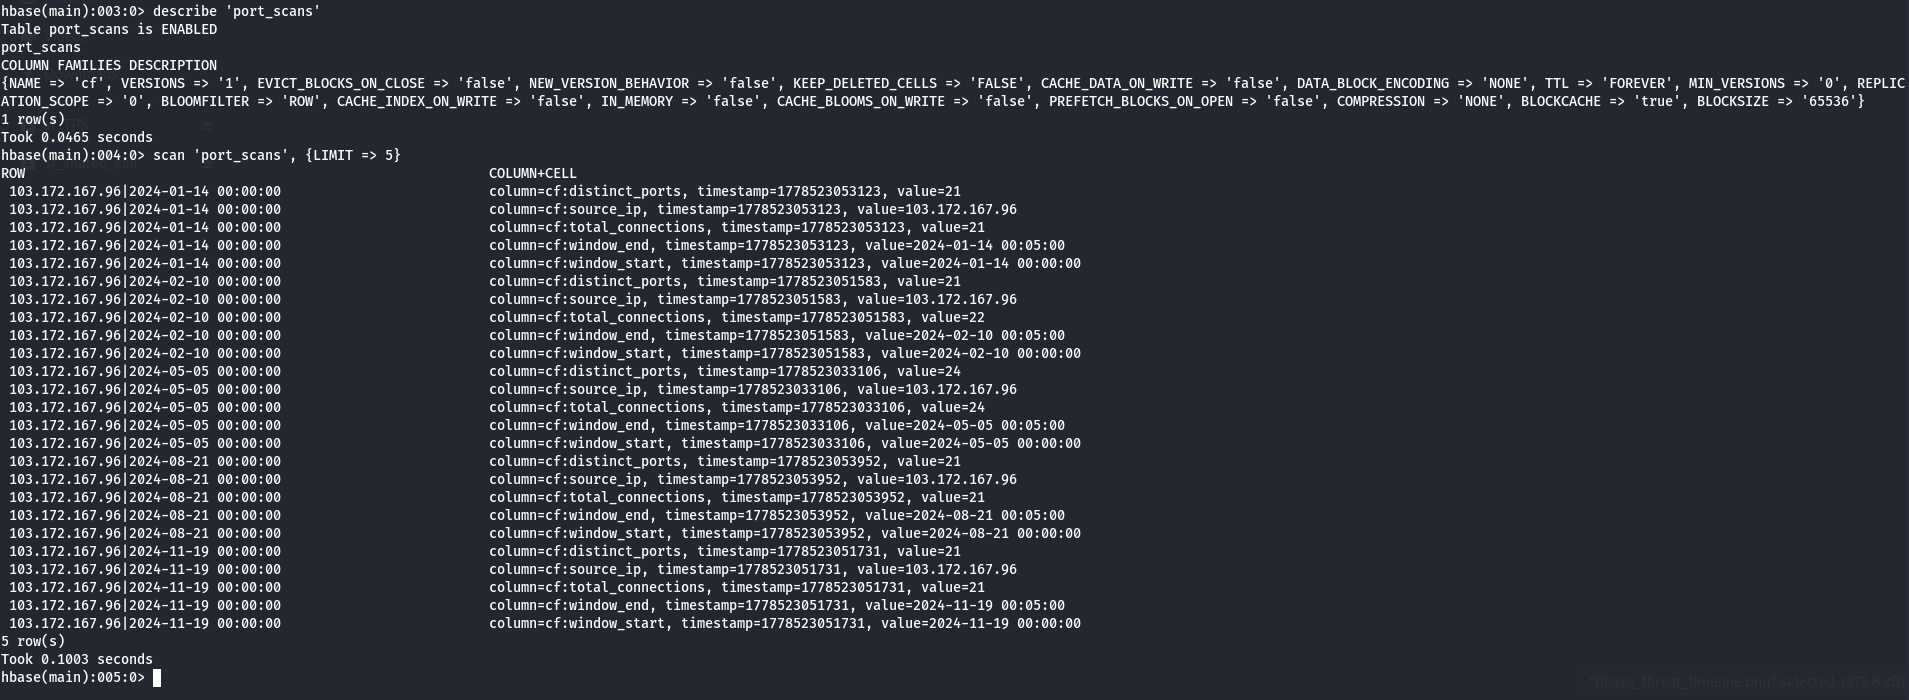
\includegraphics[width=\textwidth]{figures/batch/hbase_port_scans.png}
    \caption{Schema and sample rows of the HBase \texttt{port\_scans} table.}
    \label{fig:hbase-port-scans}
\end{figure}

\subsection{\texttt{threat\_volume}}

The \texttt{threat\_volume} table aggregates transferred bytes by threat level and highlights high-volume behaviors, notably with the 95th percentile. The expected read is by \texttt{threat\_label} in order to compare traffic volumes across threat classes.

The commands below display the schema and a sample of the stored statistics. The table contains the \texttt{avg\_bytes}, \texttt{count}, \texttt{max\_bytes}, \texttt{min\_bytes}, \texttt{p95\_bytes}, \texttt{stddev\_bytes} and \texttt{total\_bytes} aggregates by \texttt{threat\_label}.

\begin{cmdbox}
describe 'threat\_volume'\\
scan 'threat\_volume', \{LIMIT =\textgreater{} 5\}
\end{cmdbox}

\begin{figure}[H]
    \centering
    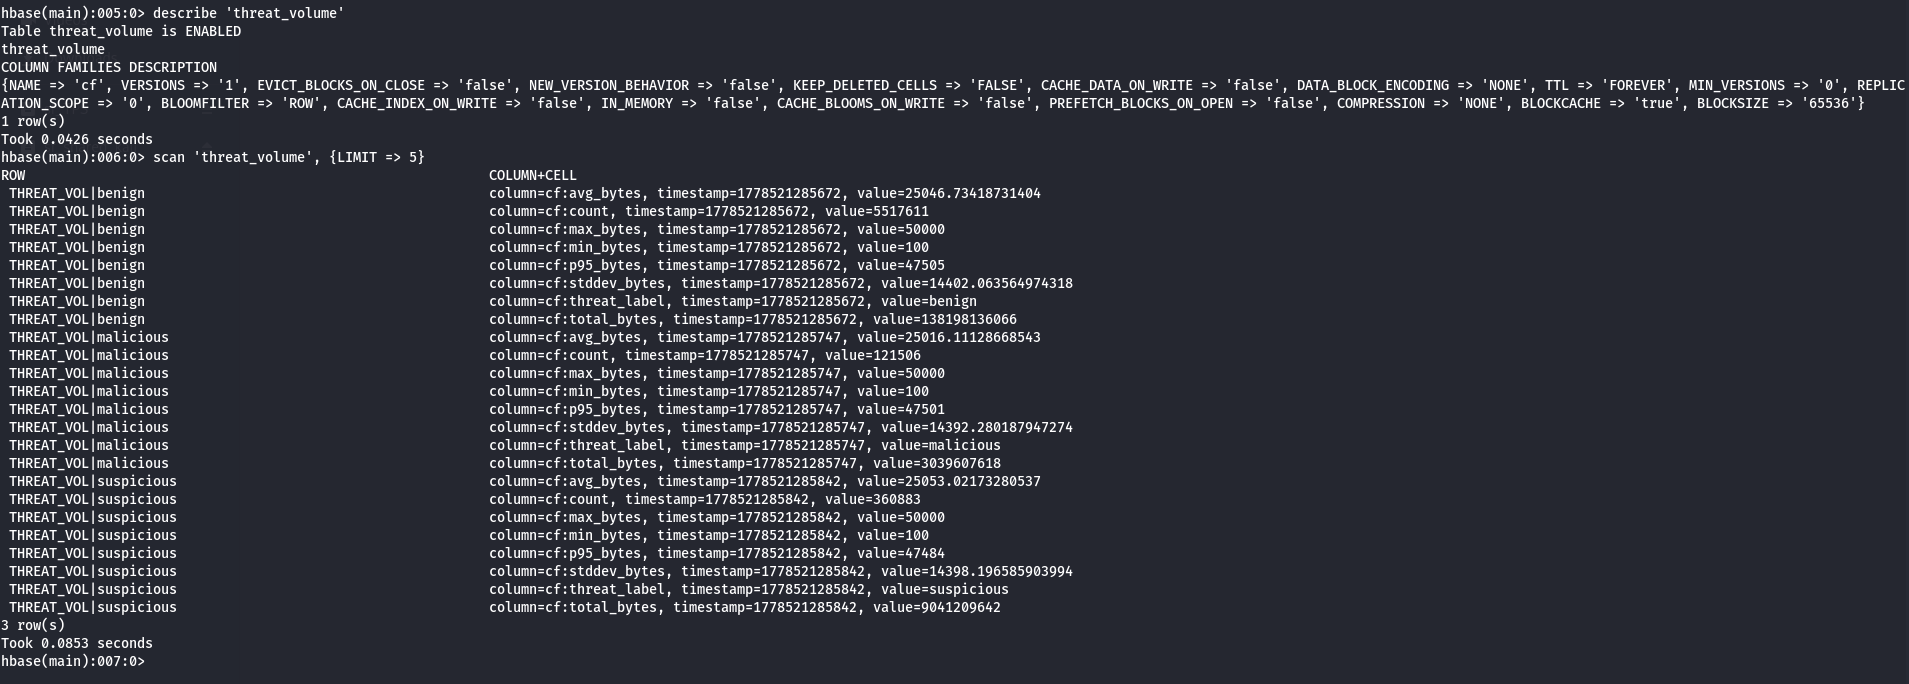
\includegraphics[width=\textwidth]{figures/batch/hbase_threat_volume.png}
    \caption{Schema and sample rows of the HBase \texttt{threat\_volume} table.}
    \label{fig:hbase-threat-volume}
\end{figure}

\subsection{\texttt{multistep\_attacks}}

The \texttt{multistep\_attacks} table is used by the \texttt{multistep\_attack\_detection.py} script. It groups IPs that appear in several stages of an attack chain: tool-based reconnaissance, SQLi exploitation and Path Traversal. The expected read is by \texttt{source\_ip} in order to identify the attack chains associated with an origin.

The obtained result validates the storage of multi-step correlations for serving. It shows columns such as \texttt{attack\_types}, \texttt{sqli\_hits}, \texttt{traversal\_hits}, \texttt{tool\_hits}, \texttt{avg\_bytes}, \texttt{malicious\_count} and \texttt{risk\_level}. Some validation screenshots may also display presentation columns such as \texttt{attack\_chain} or \texttt{ordered\_steps}, used to make the chain more readable.

\begin{cmdbox}
describe 'multistep\_attacks'\\
scan 'multistep\_attacks', \{LIMIT =\textgreater{} 5\}
\end{cmdbox}

\begin{figure}[H]
    \centering
    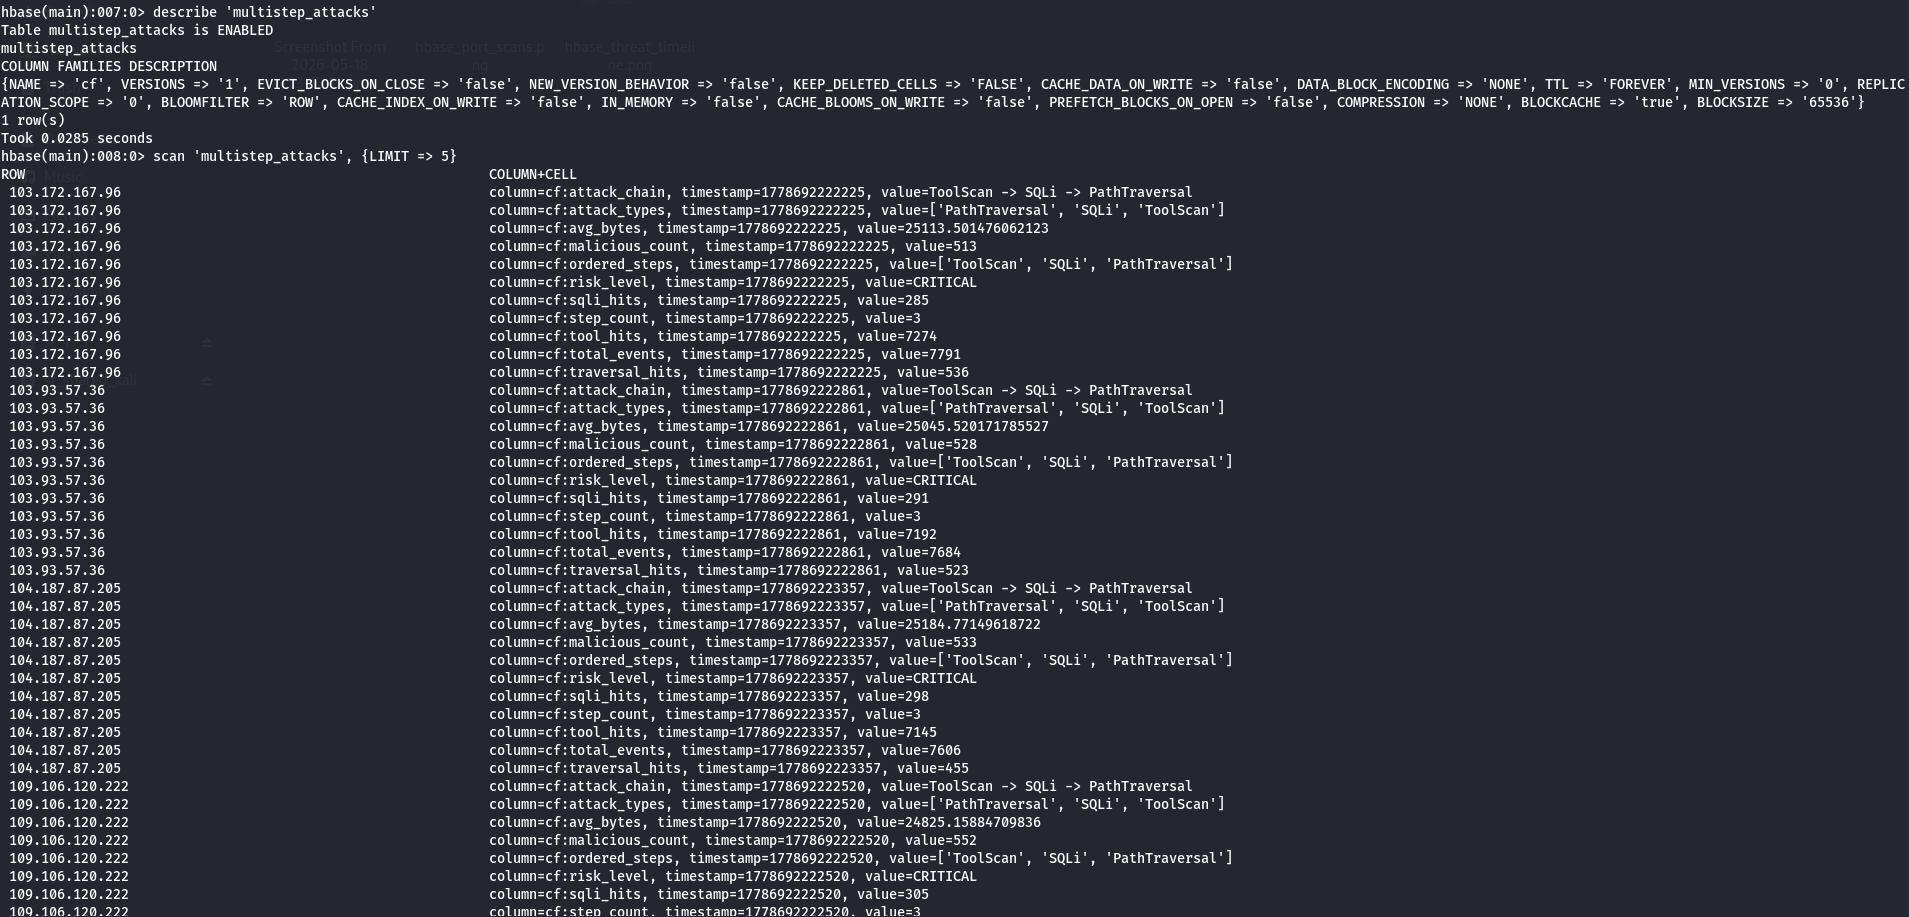
\includegraphics[width=\textwidth]{figures/batch/hbase_multistep_attacks.png}
    \caption{Schema and sample rows of the HBase \texttt{multistep\_attacks} table.}
    \label{fig:hbase-multistep-attacks}
\end{figure}

These tables do not replace \texttt{ip\_reputation}; they add specialized analytical views. They are important within Chawi's storage responsibility because they transform batch results into objects directly readable by a service: an HBase row already represents an analytical decision or a window of interest, rather than a raw event.

\section{Experimental Validation of Screenshots}

The screenshots integrated into this chapter are not decorative: they constitute an experimental validation of the storage chain. The HDFS commands confirm the existence of raw partitions and the presence of Spark batch outputs. The HBase commands validate the creation of serving tables, their schemas and the presence of sample rows. Together, these checks demonstrate that the batch results have moved from rebuildable analytical storage to serving-ready HBase views.

\section{Serving Flow between HDFS, Spark and HBase}

The batch flow follows a stable sequence. First, Spark reads the monthly HDFS partitions from \texttt{/logs/year=2024/month=XX}. Second, the job applies an aggregation or classification: IP reputation, attack patterns, timeline, port scans, volume or multi-step chains. Third, the result is written as Parquet under \texttt{/data/cybersecurity/batch}. Fourth, the metrics useful for serving are inserted into HBase through HappyBase and the Thrift port \texttt{9090}.

This model provides two advantages. On the one hand, HBase tables remain lightweight and read-oriented: they do not contain raw logs, but views prepared for the API. On the other hand, HDFS outputs remain available to verify aggregations, compare two versions of a job, or rebuild an HBase table after a schema change. Chawi therefore ensures the transition between batch analytical results and data ready to be served.

\section{Consistency with the Lambda Architecture}

The design of this batch layer reinforces the overall consistency of RAPID. HDFS guarantees reproducibility, Spark provides distributed computation, and HBase materializes historical views. Cassandra remains the operational store of the speed layer, while HBase preserves the long-term memory produced by complete processing. The API can then merge these two temporalities to provide the dashboard with a single result: recent state, historical reputation, final score and recommendation.

Thus, Chawi's contribution in \texttt{03\_batch\_layer.tex} is centered on storing and serving historical results. The HBase tables are not simple copies of files; they are read schemas designed to quickly expose batch results to the rest of the RAPID platform.

\fussy
